% ---------------------------------------------------
%
% Trabajo de Fin de Grado. 
% Author: Adriano dos Santos Moreira <alu0101436784@ull.edu.es>
% Chapter: Related Technologies
% File: Cap2_Related_Technologies.tex
%
% ----------------------------------------------------
%

\cleardoublepage
\chapter{Related Work} \label{chap:Related_Technologies}

Given the growing relevance of heterogeneous distributed memory systems and the large
development effort they pose nowadays, the research community has come up with a number of
interesting proposals to facilitate their usage \cite{Agullo:2017:Achieving, Sainz:2014:Leveraging,Lawlor:2009:Message,Stone:2010:OpenCL,Kim:2012:SnuCL}.
Although this work mainly covers the SYCL platform applied to HPC, it is also important to have an overview of the various approaches for parallel computing and related technologies.
There has been several developments in this field such as the ones cited above, although we are not going to discuss all of them.

This chapter is intended to make us aware of the general sense regarding the basic logic behind parallel oriented APIs and tools.
Inherently from one abstraction to another, we will see similarities within their core, revealing crucial mechanisms of parallel reasoning as well as establishing a connection between abstract procedures and physical parallel-oriented devices.

\section{OpenMP}
OpenMP\footnote{\href{https://www.openmp.org}{{The OpenMP API specification for parallel programming} \url{https://www.openmp.org}}} is the predominant API used to manage shared-memory parallelism used in scientific applications \cite{Luecke:2015:Fast}.
It allows for more efficient load balancing for multithreaded tasks.
This abstraction is also designed to be a flexible standard, so it becomes easy to implement on different platforms.
In essence, OpenMP extends C/C++ and Fortran with compiler directives and runtime functions that allow for a high level of parallelism expressiveness \cite{Dagum:1998:OpenMP}.
It is composed of the following basic ideas:
\begin{itemize}
    \item Control structure: Reduced amount of control structures, enough for most parallel applications.
    \item The data environment: Environment context for each process.
    \item Synchronization:
    \begin{itemize}
        \item \textbf{Explicit} synchronization using interprocess communication, which is slow.
        \item \textbf{Implicit} synchronization present when starting and finishing parallel and control constructs.
        \item OpenMP also offers different \textbf{tools for synchronization}, depending on the specific action and/or conditions, which are usually more time efficient than explicit synchronizations.
    \end{itemize}
    \item The runtime library: A miscellaneous set of mechanisms to tune an application, such as dynamically changing the number of processes used to execute parallel regions.
\end{itemize}

Listing \ref{listing:openmp-simple} presents a simple OpenMP application which runs a parallel for loop written in C++.

\lstinputlisting[language=C++,style=cppstyle,caption={Consecutive pairs average on OpenMP. \href{{https://www.openmp.org/wp-content/uploads/OpenMP3.1-CCard.pdf}}{\textit{Original source}}.},label={listing:openmp-simple}]{listings/openmp_simple.cc}

The purpose of the function is to calculate the average of each pair of consecutive elements in the \textit{a} array and store the result in the corresponding position of the \textit{b} array.
The OpenMP directive \texttt{\#pragma omp parallel for} is used to parallelize the loop.
As noted in the example code, the loop counter \textit{i} is implicitly private in OpenMP, meaning that each thread gets its own private copy of \textit{i}.

\section{HPL}

The HPL (Heterogeneous Programming Library) \cite{Viñas:2018:Heterogeneous} is a framework built on top of OpenCL that enables the exploitation of heterogeneous computing in C++.
Within HPL, the primary application operates on the host, and the code segments executed in OpenCL consist of kernel functions.
These functions can be written either directly in C++ using the HPL embedded language or in native OpenCL C.

The main functionality of this library comes with its \texttt{Array} class, which encapsulates the data to be manipulated inside of the kernels, indicating both the data type and the number of dimensions of the array.
On the other hand, scalar types should also be encapsulated within their HPL equivalent (\texttt{Float}, \texttt{Int}, etc.).
Listings from this section illustrate these ideas.

\lstinputlisting[language=C++,style=cppstyle,caption={SAXPY on HPL (HPL embedded language). \href{{https://github.com/fraguela/hpl?tab=readme-ov-file}}{\textit{Original source}}.},label={listing:hpl-saxpy-embedded}]{listings/hpl_saxpy_embedded.cc}

Listing \ref{listing:hpl-saxpy-embedded} displays how to perform a SAXPY (single precision A X plus Y) operation using the HPL embedded language.
To create a kernel we simply write a regular C++ function and use the data types provided by the library as the argument types.
To invoke the kernel, we call the \texttt{eval()} function with the kernel name as the argument followed by another call with the arguments for the execution of the kernel, as shown in Listing \ref{listing:hpl-saxpy-embedded}

Since this platform is based on OpenCL, there is a method to execute already coded OpenCL kernels.
Listing \ref{listing:hpl-saxpy-opencl} exemplifies this case.
The key difference from the former example remains on the procedure for the kernel call.
Just before the \texttt{eval()} call, we associate the OpenCL version of the kernel (specified in the \texttt{saxpy\_kernel} string) with the HPL function handle via the \texttt{nativeHandle()} function, which arguments are a function whose arguments define an equivalent version of the kernel written as specified for the HPL framework (additional details regarding the kernel behaviour can be specified), the name of the kernel function within the code and the actual OpenCL code.
\pagebreak

\lstinputlisting[language=C++,style=cppstyle,caption={SAXPY on HPL (OpenCL kernel). \href{{https://github.com/fraguela/hpl?tab=readme-ov-file}}{\textit{Original source}}.},label={listing:hpl-saxpy-opencl}]{listings/hpl_saxpy_opencl.cc}

\section{CUDA}

As presented in \cite{Liang:2011:GridCuda}, CUDA\footnote{\href{https://docs.nvidia.com/cuda}{{CUDA C++ documentation} \url{https://docs.nvidia.com/cuda}}} is a programming model and a parallel computing platform developed by NVIDIA, aimed to be used in general purpose GPUs for their CUDA-enabled GPU devices.
It was originally launched in 2007 and one of its main goals is to allow for the creation of scalable programs within the parallel computing paradigm.
To accomplish this, CUDA offers a simple yet powerful abstraction based on three key points: a hierarchy of thread groups, shared memories and barrier synchronization.

\begin{figure}[H]
	\centering
	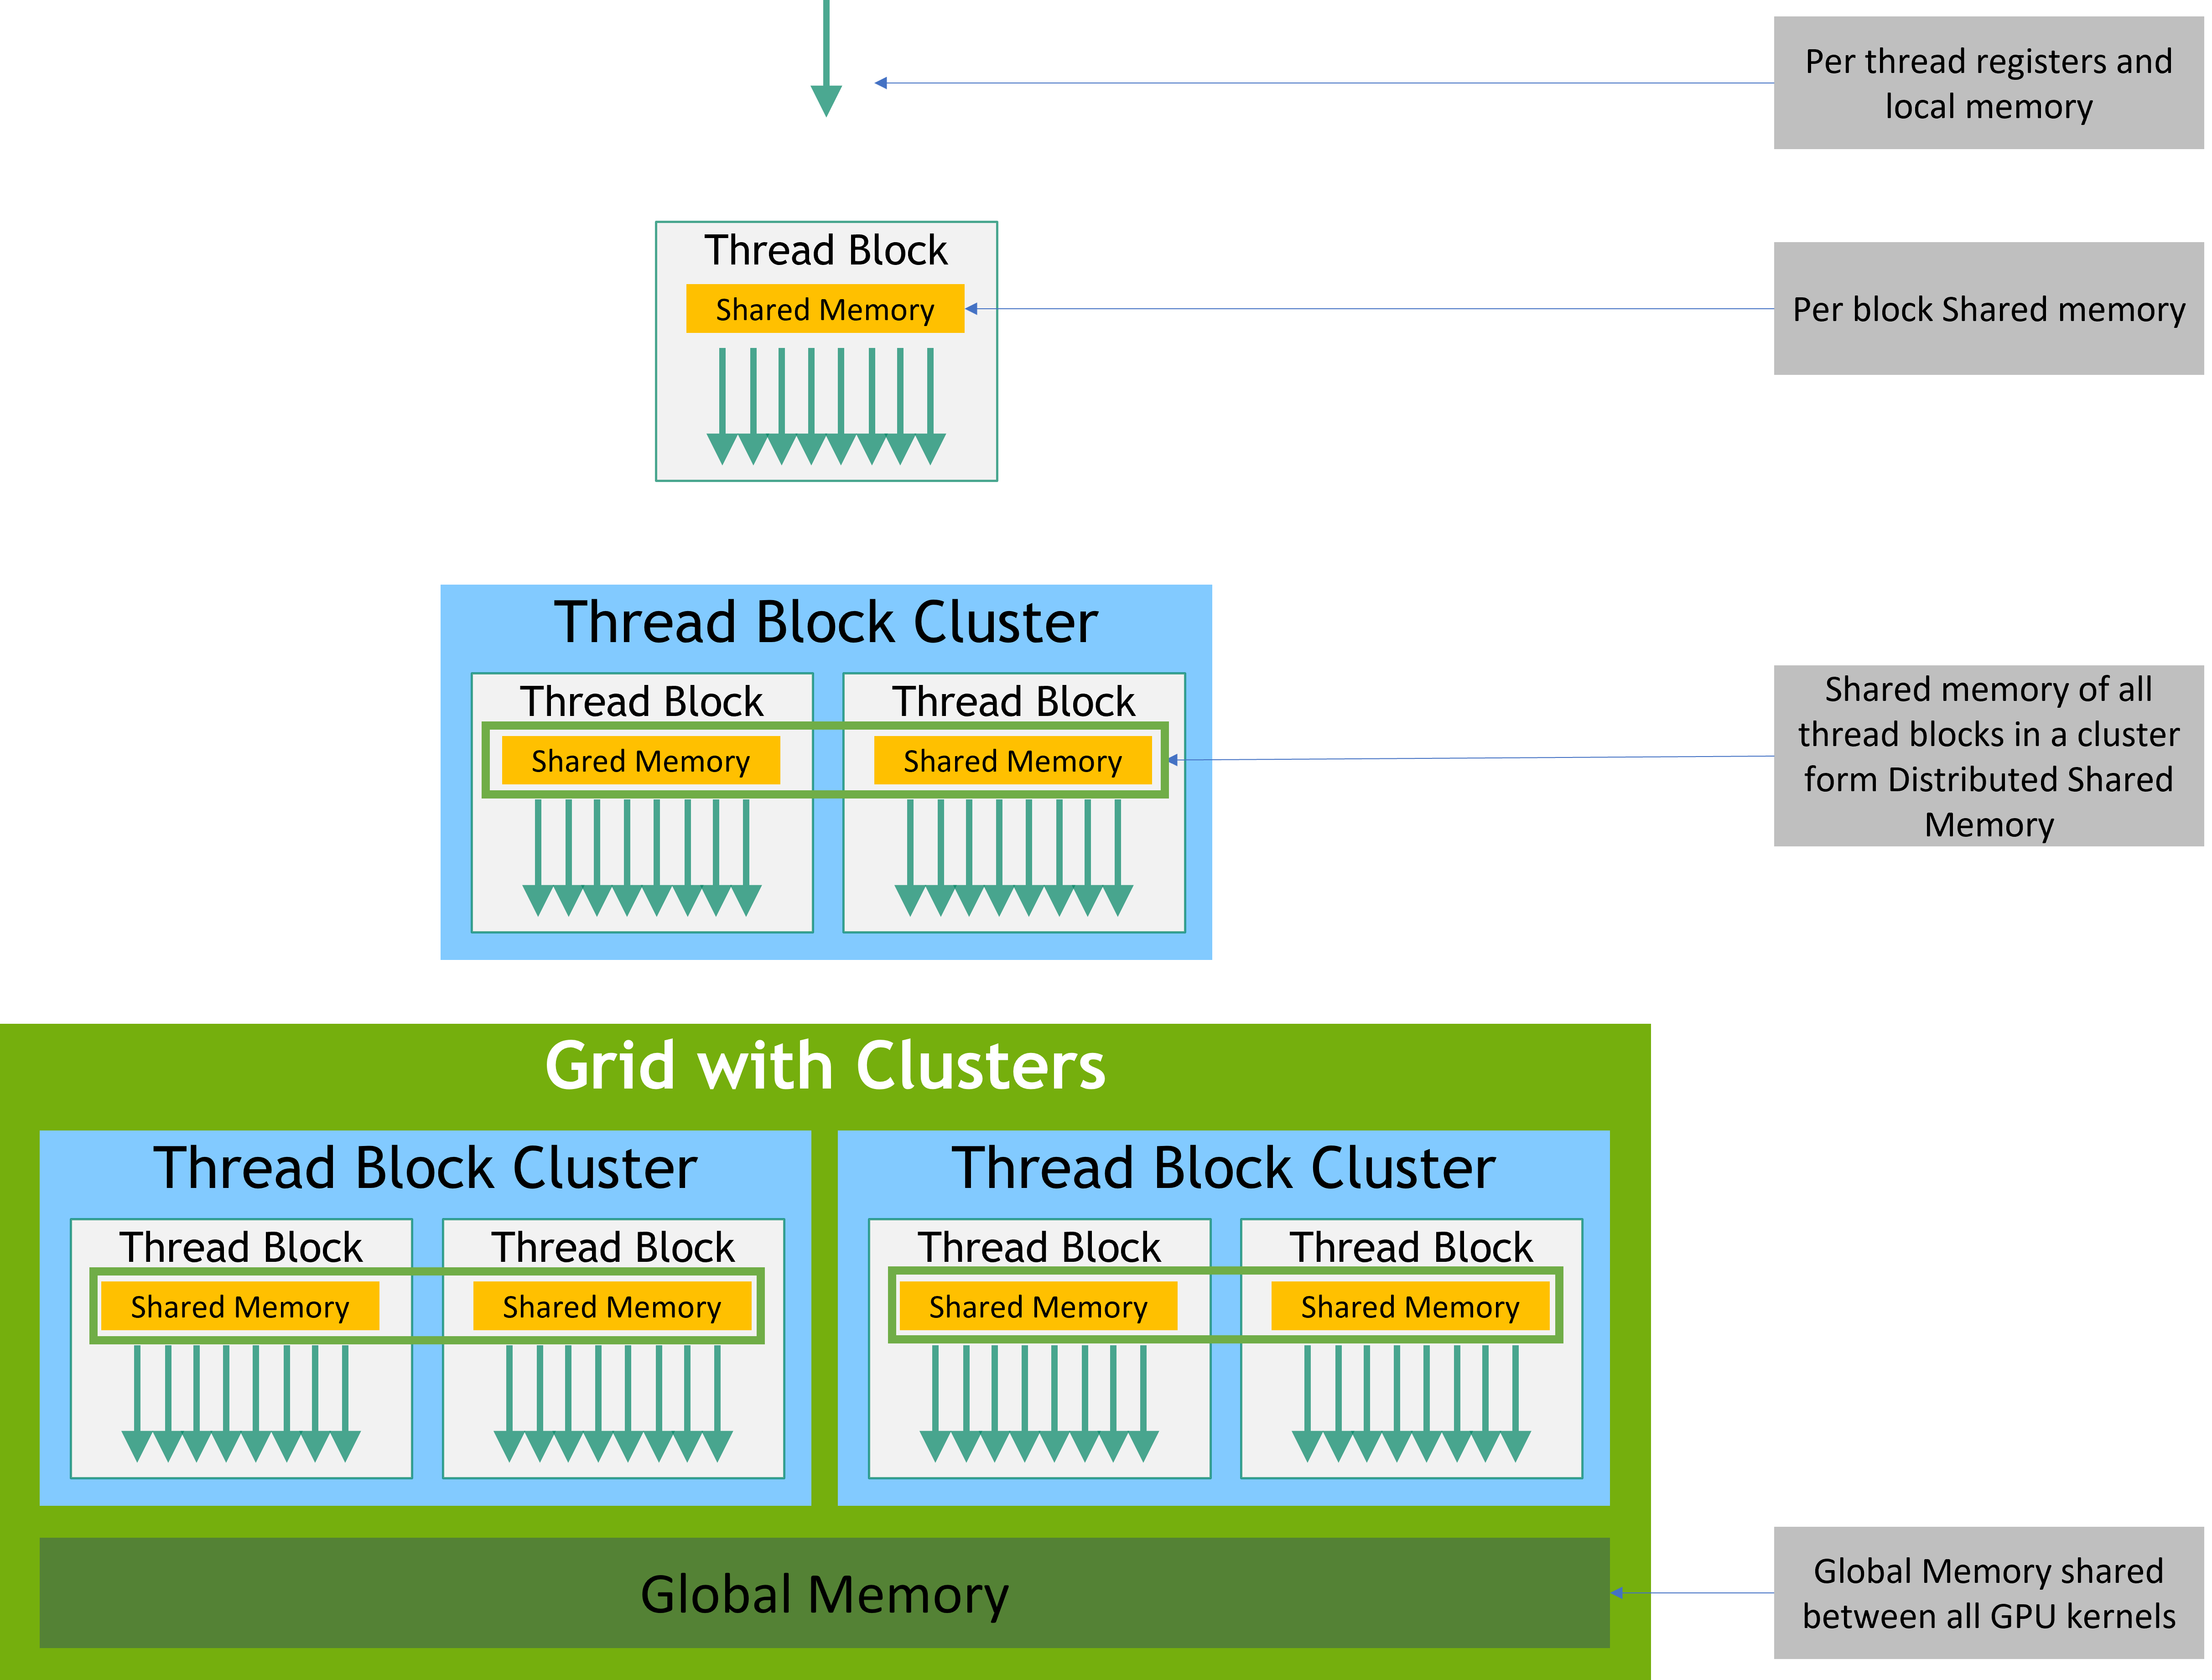
\includegraphics[width=\linewidth]{images/cuda-memory-hierarchy.png}
	\caption{CUDA memory hierarchy.}
	\label{fig:cuda-memory-hierarchy}
\end{figure}

With the CUDA platform, problems can be subdivided in blocks of threads within a grid and subproblems can be solved in parallel cooperation within a block.
The memory system in place for all of these pieces works as shown in Figure \ref{fig:cuda-memory-hierarchy}
The division in multiple independent pieces allows for scheduling on an undetermined number of GPU processors, thus enabling hardware scalability.
This platform is used broadly to solve real world problems regarding physics, biology and data mining, among others.

The CUDA platform is available on a wide variety of languages, primarily focusing on C/C++ and Fortran.
To display the basic usage and expressions for CUDA, we present in Listing \ref{listing:cuda-vector-add} an example program written in C++.
\pagebreak

\lstinputlisting[language=C++,style=cppstyle,caption={Vector add on CUDA. \href{{https://docs.nvidia.com/cuda/cuda-c-programming-guide/index.html\#kernels}}{\textit{Original source}}.},label={listing:cuda-vector-add}]{listings/cuda_vector_add.cc}

First of all, we have a declaration of a function starting with the \texttt{\_\_global\_\_} keyword, which specifies the following function as a kernel, which can only be executed on the device.
Inside of it there is the actual kernel code, in which we can highlight the use of \texttt{threadIdx}, a 3-dimensional vector which identifies the working thread.

Similarly, we have \texttt{blockIdx} that provides a unique identification for thread blocks.
On the other hand, inside of the main function there is a kernel invocation.
This asynchronous call comes with execution configuration denoted by \texttt{<}\texttt{<}\texttt{<1, N>}\texttt{>}\texttt{>}, in which the first parameter specifies the number of blocks and the second specifies the number of threads per block.
Both of which can be simple integers or \texttt{dim3} values to indicate these are multidimensional entities.

\section{OpenCL}

OpenCL is an open standard designed for general-purpose parallel programming on multi-core architectures \cite{Viñas:2018:Heterogeneous, Reyes:2012:Directive}.

It addresses a wide range of applications and acts as an efficient, low-level programming interface. The goal of OpenCL is to establish itself as the foundation platform for a parallel computing ecosystem.
OpenCL aims to be a tool to produce portable yet efficient code.
There is a clear division of ideas that comprehend the standard, which is composed of the models: Platform, Memory, Execution and Programming.
These are explained in further detail in the reference above.
Following, we have an overview of the OpenCL functionality.

\begin{figure}[H]
	\centering
	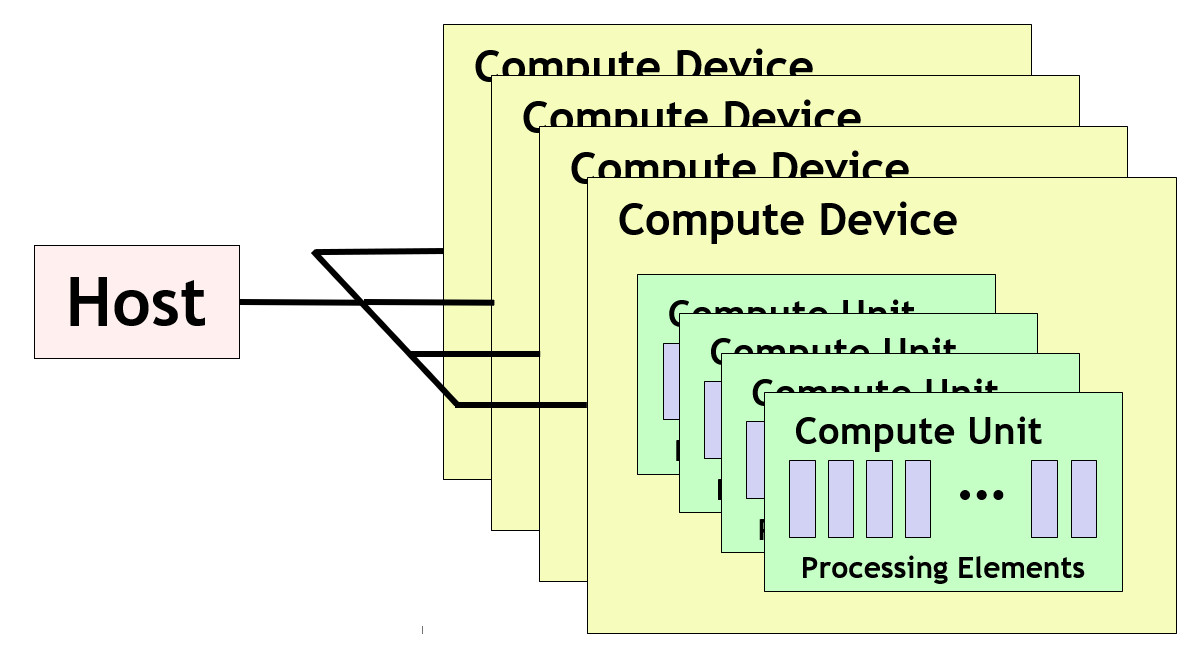
\includegraphics[width=0.7\linewidth]{images/opencl_platform_model.jpg}
	\caption{OpenCL platform model.}
	\label{fig:opencl-platform-model}
\end{figure}

As we can see in Figure \ref{fig:opencl-platform-model}, an OpenCL host is connected to one or more OpenCL devices, which in turn are composed of one or more compute units (CU).
Such units are subdivided in one or more processing elements (PEs).
The PEs are the ones in charge of executing actual code.

The way an OpenCL application operates is by running the host program on the host platform, which is in charge of defining the kernel contexts and managing kernel executions, whilst submitting commands from it to execute kernels on the devices.

Similarly to CUDA, kernels are scheduled to run under a defined index space, meaning that each kernel instance has a specific identification, which determines how the kernel will execute.

\begin{figure}[H]
	\centering
	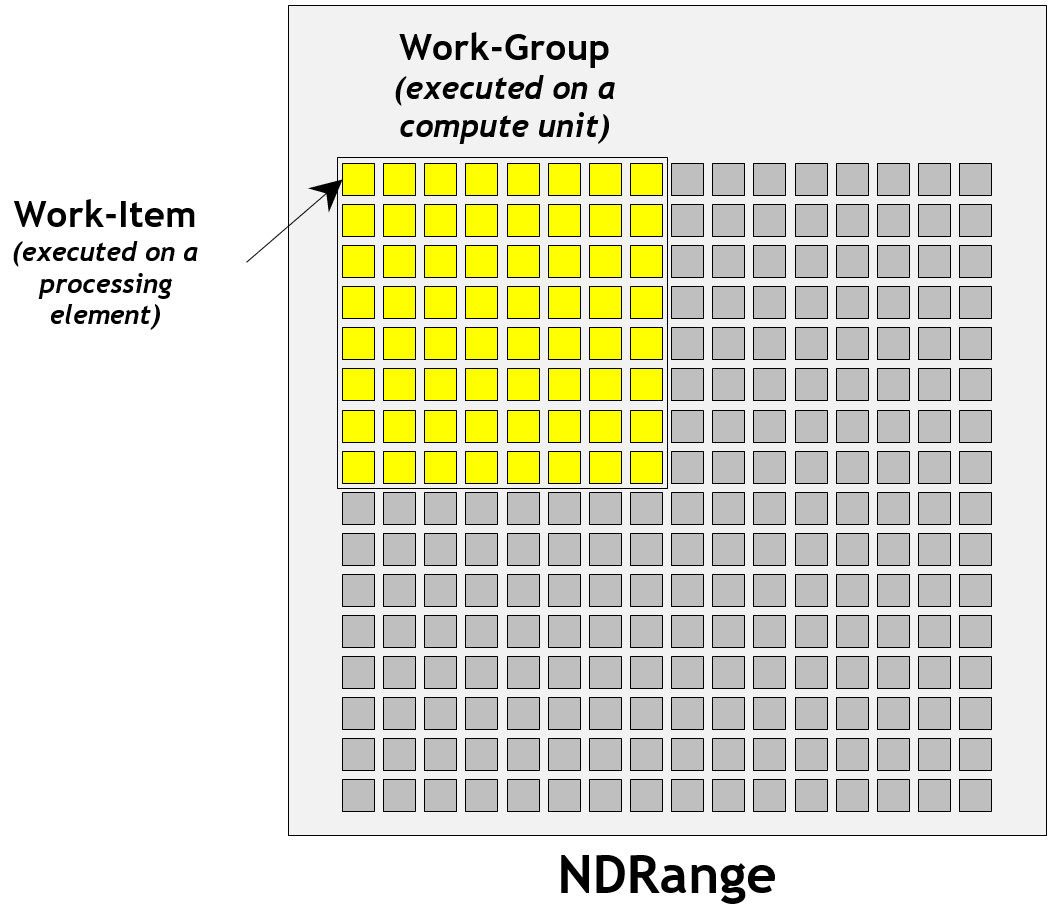
\includegraphics[width=0.75\linewidth]{images/opencl-ndrange.jpg}
	\caption{OpenCL NDRange.}
	\label{fig:opencl-ndrange}
\end{figure}

A PE is responsible for the execution of a work-item, which is encompassed within a work-group, as we can see in Figure \ref{fig:opencl-ndrange}.
This coarse-grained composition allows for the execution of different strategies when using the index space.
Furthermore, the idea of a N-dimensional index space (NDRange), where N is one, two or three, gives users high flexibility to refine their works.
This abstraction shapes the indexes used in the work-items, affected by the dimensionality and work group divisions as well.

\section{Directive-based Languages for Accelerators}

In \cite{Grillo:2013:PGD}, the authors present the most relevant approaches that have been used to leverage heterogeneous architectures using languages enhanced with the use of specific directives.

We will now review the most significant of these approaches.

\subsection{OpenMPC - OpenMP Extended for CUDA}

OpenMPC \cite{Lee:2010:OpenMPC} is an abstraction of the CUDA programming model built on OpenMP.
OpenMPC performs a translation from OpenMP to CUDA with the addition of special directives and variables, which are used to make CUDA-specific optimizations.
There is an extensive set of clauses and environment variables.
Examples of some of these clauses are:
\begin{itemize}
    \item \texttt{maxnumofblocks(N)}: Specifies the maximum number of thread blocks for a kernel.
    \item \texttt{threadblocksize(N)}: Specifies the thread block size for a kernel.
\end{itemize}
The translation from OpenMPC to CUDA starts by analyzing the code and passing the result to the OpenMP to CUDA translator, which performs the actual translation aided by the optimization information obtained from the previous step.

\subsection{hiCUDA}

hiCUDA \cite{Han:2011:hiCUDA} is a high-level abstraction layer built on top of CUDA.
It provides an easy to use interface that solves mechanical tasks for the development of CUDA programs.
An important highlight that motivates the use of hiCUDA is the fact that the process of migration from existing code to CUDA may be challenging, as evidenced by the need for programmers to manually handle intricate tasks such as managing data transfers between host and GPU memories, and optimizing GPU memory utilization.
These tedious tasks are alleviated by the automated work that hiCUDA can offer.

This tool can extract kernels from their original source and decide how to allocate the work threads and blocks according to user defined configuration clauses.
This is accomplished using special hiCUDA directives, which would then be translated to actual CUDA code.
The authors have developed a prototype of this idea which does exactly that.
Is also important to note that the same source files of a hiCUDA project can be used to create both sequential and GPU versions of the code.

\subsection{PGI Accelerator Model}

The PGI Accelerator Model \cite{Portland:2010:PGI} was created by The Portland Group for the Fortran and C languages.
It is essentially a set of directives designed to guide the compiler in creating kernels and regions of code that can be offloaded to an accelerator device.
This model allows for portability across multiple operating systems, various accelerators and types of host CPUs.

The main functionality is provided by the \texttt{acc region} directive, which specifies a region within the code that contains a parallel loop kernel.
Most of the directives provided by this model are optional, and are mostly used to improve performance based on compilation hints.
On the other hand, this abstraction offers implicit mechanisms such as data flow and array region analysis to determine when data transfers between host and device should occur, as well as accelerator startup and shutdown, among other uses.

\subsection{OpenACC}

Considering the OpenACC standard, the ULL GCAP\footnote{\href{https://portalciencia.ull.es/grupos/6369/detalle}{{ULL GCAP} \url{https://portalciencia.ull.es/grupos/6369/detalle}}} research group (\textit{High Performance Computing Group}) developed their own version of the compiler, called \texttt{accULL} \cite{Reyes:2012:Directive}, standing as one of the few available implementations of the OpenACC standard.
OpenACC shares an important piece of the high-level features present in the PGI Accelerator Model, it is based on directives that indicate regions of code that could be run on an accelerator device.
This abstraction frees the developer from writing device specific code details, allowing them to focus on other tasks.
The main \textit{pragma} regions supported by OpenACC are the following:
\begin{itemize}
    \item \texttt{data}: Specifies data regions.
    \item \texttt{kernels}: Groups of loop nests that can be executed on the devices.
    \item \texttt{parallel}: Similar to \texttt{kernels} but allows for better control over the code.
\end{itemize}

There are other annotation mechanisms to further tailor the execution and behaviour of OpenACC such as clauses that can reduce memory transfers like \texttt{copy\_in} or \texttt{copy\_out}.
